\chapter{Probabilistic Generative Models}
\label{ch:generative_models}

Probabilistic generative models (PGMs) are a class of models that either aim to learn the underlying probability distribution of a dataset or at least facilitate means to generate new samples indistinguishable from the data.
It is worth highlighting that there is conflicting terminology and many overlapping definitions in the field of PGMs~\cite{DiscriminativeVsGenerative, MachineLearningDiscriminative}, so we will attempt to directly define the terms used in this thesis.

We assume the existence of some unknown probability density $p_\X(\x): \mathcal{X} \rightarrow \mathbb{R}$ over some random variable $\X \in \mathcal{X}$ which is used to populate the training set $\mathcal{D} = \{\x_i\}_{i=1}^N$.
A PGM with parameters $\theta$ fit using $\mathcal{D}$ allows for the generation of new samples following a close approximation of $p_\X(\x)$, denoted as $p_{\theta}(\x)$.
There exist many types of PGMs; some models such as Normalizing Flows (NFs)~\cite{VariationalInferenceNormalizing} provide an explicit functional form for the density $p_{\theta}(\x)$, while others like Generative Adversarial Networks (GANs)~\cite{GenerativeAdversarialNetworks} implicitly learn the density and only permit sampling from it.

We are often interested in approximating a conditional distribution $p_{X}(\x|\con)$ where $\con$ is some context variable.
Supervised learning can also be described in the framework of conditional generation where, in contrast to the notation in \Cref{sec:supervised_learning}, $\x$ is the target variable, and $\con$ is the input.

This section covers the theory behind the PGMs used elsewhere in this thesis, namely NFs and diffusion models.
These models are nominally used to generate continuous data, which matches much of the data we are interested in generating in the context of HEP.
Generative models on discrete data, such as the autoregressive models used in text generation~\cite{GPT2}, are omitted.
An overview of the models is given in \Cref{fig:generative_models}.

\begin{figure}[ht]
    \centering
    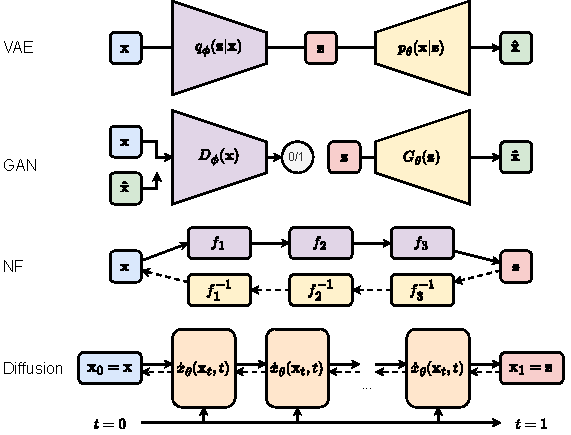
\includegraphics[width=0.8\textwidth]{Figures/generative_models/pgms.pdf}
    \caption{An overview of the generative models covered in this chapter.}
    \label{fig:generative_models}
\end{figure}


\section{Older PGMs}

Over the course of completing this thesis, the field of generative models has seen rapid development.
At the start of this thesis, applications PGMs in HEP mainly involved Variational Autoencoders~\cite{AutoEncodingVariationalBayes} (VAEs) and GANs~\cite{GenerativeAdversarialNetworks}.
While these older models produced impressive results in select domains, the generation quality and fine control we see today in state-of-the-art text-to-image~\cite{SD3, Dalle, Imagen,flux2024github} and text-to-video~\cite{ImagenVideo} models would have been inconceivable a few years ago.
The current landscape of text-to-image~\cite{Imagen, Dalle, SD3}, and even text-to-video~\cite{ImagenVideo} generation would have been inconceivable just a few years ago.
While it is remarkable how quickly the focus on VAEs and GANs has moved on, it is still important to highlight them here for historical context and to better understand the strengths of the models that have replaced them.

\subsection{Variational Autoencoders}

VAEs were introduced in 2013~\cite{AutoEncodingVariationalBayes} and quickly became a popular model for generative tasks, unsupervised learning, and variational inference.
A VAE is an example of a latent variable model.
Here, one introduces a random latent variable $\Z \in \mathcal{Z}$ which one marginalizes over to obtain the distribution of the data,
\begin{equation}
    p_\X(\x) = \int p_{\X,\Z}(\x, \z)\diff\z = \int p_\X(\x|\z)p_\Z(\z)\diff\z.
\end{equation}
The latent space usually covers all real values, $\mathcal{Z} = \mathbb{R}^d$, and the prior $p_\Z(\z)$ is taken to be a simple distribution, such as a diagonal Gaussian $\normal$.
A simple distribution is one that is easy to sample from and the density is easy to calculate.
Practically, we would like to avoid imposing what information is stored in the latent variable.

The standard choice for modelling the likelihood is to use a parametrized Gaussian with constant variance,
\begin{equation}
    p_\X(\x|\z) \approx p_{\theta}(\x|\z) = \mathcal{N}(\x; G_{\theta}(\z), \sigma^2 I),
\end{equation}
where $G_{\theta}$ is a neural network called the decoder.
VAEs introduce an additional parametrized distribution to approximate the posterior which is also taken to be Gaussian with a diagonal covariance matrix,
\begin{equation}
    p_\Z(\z|\x) \approx q_\phi(\z|\x) = \mathcal{N}(\z; \boldsymbol{\mu}_\phi(\x), \boldsymbol{\Sigma}_\phi(\x)).
\end{equation}
Here the estimation of the mean and variance of the approximate posterior is done by a neural network called the encoder and gradients are backpropagated through the stochastic latent variable using the reparametrization trick~\cite{AutoEncodingVariationalBayes}.

One can not train this model by simply maximizing the likelihood of the data, as this is intractable.
However, this form sets up a mapping between the data space to the latent space and back again, and one can train the model by maximizing the evidence lower bound.
Practically, this involves minimizing two terms, the reconstruction loss and the KL-divergence between the approximate posterior and the prior,
\begin{equation}
    \mathcal{L}(\theta, \phi) = \mathbb{E}_{\z \sim q_{\phi}(\z|\x)}[||\x - G_{\theta}(\z)||^2] - \beta D_{KL}(q_{\phi}(\z|\x) || p_\Z(\z)),
\end{equation}
where $\beta$ is a hyperparameter that balances the two terms~\cite{BetaVAE}.

Typically, the dimensionality of the latent space is much lower than that of the data space, so the information bottleneck means the model is forced to learn a compressed representation.
VAEs are simple to train but have several limitations.
The bottleneck means that high-frequency detail is dropped, resulting in low-quality samples.
The model is also sensitive to the tuning of $\beta$, often leading to a collapse into one of two regimes.
Either the prior loss dominates, all samples are encoded to the same Gaussian, and all information is lost, or the reconstruction loss dominates.
In the latter case, the learned posterior $q_\phi(\z)$ is non-Gaussian, and extra steps are required to sample from it, such as fitting a kernel density estimator to the empirical distribution of the latent variables~\cite{KDEVAE}.

Conditional information can be injected into the VAE simply by combining the context variable with both the inputs to the encoder and decoder.
The compression of the latent means that it should only store orthogonal information to the context variable, which is useful for disentanglement~\cite{cVAE}.

VAEs were never particularly good at generating high-quality samples, but attempts were still made in HEP to use them for fast simulation of detector responses~\cite{VariationalAutoencodersJet, GraphVariationalAutoencoder, ParticlebasedFastJet}.
They were also used for anomaly detection~\cite{VariationalAutoencodersAnomalous, DeepSetVAE, MassiveIssueAnomaly}.
These applications produced mixed results, and the field has moved on to more powerful models.

\subsection{Generative Adversarial Networks}

Until recently, GANs were the state-of-the-art generative models for producing high-quality samples, most notably demonstrated in generating high-resolution images~\cite{StyleGAN2, StyleGAN3}.
GANs are based on a two-player min-max game between a generator $G_\theta(\z)$ and a discriminator $D_\phi(\x)$, each a neural network with parameters $\theta$ and $\phi$ respectively.
These networks compete in a zero-sum game in which one network's loss is the other's gain.

The generator takes a random latent sample $\z \sim p_\Z(\z)$ and returns a synthetic sample $\hat{\x} = G_\theta(\z) \in \mathcal{X}$.
The discriminator takes samples from both the training set and the synthetic samples and returns a probability that the sample is from the training set, $D_\phi(\x) \in [0, 1]$.
The generator aims to fool the discriminator into thinking the generated samples are real.
Given powerful enough networks, the unique Nash equilibrium of this game is a generator that reproduces the true data distribution and a uniform discriminator output for all samples.

This game has many variations for defining the specifics and loss terms.
The most widely used is the original non-saturating GAN~\cite{GenerativeAdversarialNetworks}.
This loss requires two passes through each network, one to update the discriminator and one to update the generator.
\begin{align}
    \mathcal{L}_{\text{D}}(\phi)   & = -\mathbb{E}_{\x \sim \mathcal{D}}[\log D_{\phi}(\x)] - \mathbb{E}_{\z \sim p_\Z(\z)}\log(1 - D_{\phi}(G_{\theta}(\z))], \\
    \mathcal{L}_{\text{G}}(\theta) & = -\mathbb{E}_{\z \sim p_\Z(\z)}[\log D_{\phi}(G_{\theta}(\z))].
\end{align}
Other variants that use different loss derivations exist, such as the Wasserstein GAN~\cite{WGAN1} and the Geometric GAN~\cite{GeometricGAN}.
There is plenty of literature on which variants are best suited for different tasks and which converge to the desired Nash equilibrium~\cite{WhichTrainingMethods}.

The main drawback of GANs is that they are challenging to train.
Often, mode collapse occurs, where the generator exploits a weakness in the discriminator and produces the same samples repeatedly.
Many tricks are required to stabilize training~\cite{WhichTrainingMethods}, such as minibatch discrimination~\cite{ProGAN} and gradient penalties~\cite{WGAN}.
Another drawback to GANs is that it is challenging to produce a conditional generator $G_\theta(\x|\con)$.
Simply concatenating the context variable to both the generator and discriminator inputs leads to mixed results, and the generator is prone to ignoring the context variable~\cite{cGAN}.

In HEP, GANs have mainly been trialled as a method for fast simulation~\cite{MPGAN, GAPT, CaloGAN, EPICGAN}.
However, the main issue is that GANs tend not to cover the full data distribution.
Most of the generation we are looking for in fast simulation is conditional, as detector response depends on the properties of the incoming particle, making GANs not optimal for this task.

\section{Normalizing Flows}
\label{sec:flows}

NFs are a popular tool for both variational inference~\cite{VariationalInferenceNormalizing, NormalizingFlowsProbabilistic}
and density estimation~\cite{NICENonlinearIndependent}.
Like GANs and VAEs, they prescribe a method to train a transformation from a simple latent distribution into one that matches the data.
However, unlike GANs and VAEs, NFs allow for explicit likelihood evaluation, making them much easier to train and well-suited for density estimation.

At the core of NFs is the change of variables formula.
Given two random variables $\X$ and $\Z$ with equal dimensionality related by a diffeomorphism $f: \mathcal{X} \rightarrow \mathcal{Z}$, the probability densities $p_\X(\x)$ and $p_\Z(\z)$ are related by,
\begin{equation}
    \label{eq:change_of_variables}
    p_\X(\x) = p_\Z(f(\x)) \left|\det D f(\x) \right|.
\end{equation}
Here, $f(\x)$ is a differentiable bijective function with a differentiable inverse, otherwise known as a diffeomorphism, and $D f(\x)$ is the Jacobian of the transformation.
The density $p_\X(\x)$ is called a \textit{pushforward} of the density $p_\Z(\z)$ by the function $f$, $p_\X = f_\# p_\Z$.

NFs constructs explicit approximations of data density by defining it as a pushforward of the latent through a parametrized neural network,
\begin{equation}
    p_{\X}(\x) \approx p_{\theta}(\x) = f_{\theta \#} p_\Z(\z) = p_\Z(f_{\theta}(\x)) \left|\det D f_{\theta}(\x) \right|.
\end{equation}
The neural network $f_{\theta}$ must be a diffeomorphism, placing restrictions on the architecture of the network.

Like all neural networks, NFs are built from the composition of several simple layers $f_\theta = f_{\theta_1} \circ f_{\theta_2} \circ \ldots \circ f_{\theta_L}$.
Unlike other neural networks, each \textit{flow layer} has to be a diffeomorphism, as the composition of two diffeomorphisms is itself a diffeomorphism.
The Jacobian of the full transformation is simply the product of the Jacobians of the individual layers,
\begin{equation}
    f_\theta = f_{\theta_1} \circ f_{\theta_2} \circ \ldots \circ f_{\theta_L} \quad \Rightarrow \quad \det D f_\theta(\x) = \prod_{i=1}^L \det D f_{\theta_i}(\x_i).
\end{equation}
This composition property allows us to construct arbitrarily complex transformations, allowing for the approximation any data distribution~\cite{bogachev2005triangular}, using a finite number of layers.

NFs are typically trained via a maximum log-likelihood approach, or more specifically, they use a negative log-likelihood loss function,
\begin{equation}
    \label{eq:nf_loss}
    \begin{aligned}
        \mathcal{L}(\theta)
        \frach & = \mathbb{E}_{\x \sim \mathcal{D}}[-\log p_{\theta}(\x)]                                                                        \\
        \frach & = \mathbb{E}_{\x \sim \mathcal{D}}\left[-\log p_{\Z}(f_{\theta}(\x)) - \log \left|\det D f_{\theta}(\x) \right|\right]          \\
        \frach & = \mathbb{E}_{\x \sim \mathcal{D}}\left[-\log p_{\Z}(f_{\theta}(\x)) - \sum_{i=1}^L \log \left|\det D f_i(\x_i) \right|\right].
    \end{aligned}
\end{equation}
Note that due to the Jacobian's composition property, the log determinant term is a sum of the log determinants of the individual layers, leading to essentially independent contributions per layer in the final loss.

During training, the flow is said to run in \textit{forward-mode}, transforming samples from the data space to the latent space.
Once the model is trained, it can again be used in forward-mode to yield the density at any measured point, or it could be run in \textit{reverse-mode} $f^{-1}$ to generate samples from the data distribution.

Conditional density estimation is a natural extension of NFs.
The only modification is that the context variable is included in the input of each layer in the flow.
This allows the model to learn the conditional distribution $p_{\X}(\x|\con)$ and yields surprisingly good results and highly calibrated uncertainties that match the aleatoric uncertainty in the data almost exactly~\cite{SolvingInverseProblems, InferenceAstrophysicalParameters, ComposingNormalizingFlows, NormalizingFlowsProbabilistic}.
Standard regression, which operates under the assumption of a Gaussian likelihood, is often overly restrictive.
A more effective approach for almost all regression tasks involves framing them as conditional density estimation, where NFs emerge as one of the most suitable tools.

While NFs allow for the exact calculation of the likelihood, they are not without their drawbacks.
The main issue is that NFs are computationally expensive and do not scale well to high-dimensional data.
Even with the specialized flow layers explained in the next section, the complexity of calculating the Jacobian determinant is prohibitive for data with more than a few hundred dimensions.
As NFs describe continuous morphs of data if the latent distribution is connected, so will any learned density.
This causes issues when attempting to model data with disconnected support.
Discrete data needs to be \textit{dequantized} before being fed into the flow to prevent singularities from occurring during training, a notable feature in image modelling where pixel values tend to be quantized to 8-bit integers~\cite{FlowImprovingFlowBased}.

These types of networks have successfully applied to collider physics, with notable applications including event generation~\cite{EventGen}, template construction~\cite{ANODE, CATHODE, CURTAINs}, unfolding~\cite{PartonsAndBack}, and detector simulation~\cite{CaloFlow2}.

\subsection{Flow Layers}

Building an NF requires stacking multiple diffeomorphism flow layers together.
They must operate on real-valued tensors $\x \in \mathbb{R}^d$ and optionally include $\con \in \mathbb{R}^c$.
In addition, for practical applications, each layer needs to be efficient to process, both in the forward- and reverse-modes, and the Jacobian determinant should be easy to compute.
The design of these layers is the core research problem in normalizing flows.

At the time of writing, the most popular flow layers are linear flows, coupling flows autoregressive flows, and residual flows.
We describe the ones most relevant to this thesis.

\subsubsection{Linear Flows}

A straightforward, non-resizing linear transform is an example of a flow layer $f(\x) = \W\x + \bias$.
Here, the inverse is simply $f^{-1}(\z) = \W^{-1}(\z - \bias)$.
Only a small amount of reparametrization is required to ensure that the matrix $\W$ is non-singular and thus invertible.
Linear flows are, however, limited in their expressiveness.
Furthermore, the complexity of calculating $\det D f(\x) = |\det \W|$ is $\bigO(d^3)$, making them computationally expensive for high-dimensional data.

One can restrict the form of the matrix to make it easier to use, as shown in \Cref{tab:linear_flows}.
The most popular choices are the LU-Factorisation and, for images, a $1\times1$-convolution~\cite{GlowGenerativeFlow}.

\begin{table}[h!]
    \centering
    \caption{Complexity of using different forms of linear flows.}
    \label{tab:linear_flows}
    \begin{tabular}{ccc}
        \toprule
        \textbf{Type}      & \textbf{Inverse}    & \textbf{Determinant} \\
        \midrule
        Full               & $\bigO(d^3)$        & $\bigO(d^3)$         \\
        Diagonal           & $\bigO(d)$          & $\bigO(d)$           \\
        Triangular         & $\bigO(d^2)$        & $\bigO(d)$           \\
        Block (c) Diagonal & $\bigO(c^3d)$       & $\bigO(c^3d)$        \\
        LU Factorized      & $\bigO(d^2)$        & $\bigO(d)$           \\
        1x1 Convolution    & $\bigO(c^3 + c^2d)$ & $\bigO(c^3)$         \\
        \bottomrule
    \end{tabular}
\end{table}

\subsubsection{Coupling Flows}

Coupling flows~\cite{NICENonlinearIndependent} describe a general approach to constructing highly expressive non-linear flows.
In a coupling flow, the input $\x$ is partitioned into two disjoint components $(\x_A, \x_B)$.
$\x_A$ is used to compute the parameters of a bijective transformation called the coupling function $h(\cdot; \phi)$ which is applied to only $\x_B$.
This can be expressed as,
\begin{equation}
    \label{eq:coupling_flow}
    f(\x) = (\x_A, h(\x_B; \phi(\x_A))).
\end{equation}
As shown in \Cref{fig:coupling_flow}, this layer is entirely reversible so long as the coupling function is invertible, whereas the conditioner $\phi$ does not have this restriction.
Additionally, the Jacobian of the transformation is a block matrix given by,
\begin{equation}
    D f(\x) = \begin{pmatrix}
        \mathbb{I}                                         & 0                                                  \\
        \frac{\partial h(\x_B; \phi(\x_A))}{\partial \x_A} & \frac{\partial h(\x_B; \phi(\x_A))}{\partial \x_B}
    \end{pmatrix}.
\end{equation}
When calculating the determinant, the entire bottom left block can be ignored, making it simply the determinant of the invertible transformation $h$.
Thus, $\phi$ can be arbitrarily complex without impacting the convertibility or the computational complexity of calculating the likelihood contributions of the layer.
It is common, therefore, to use a deep neural network for $\phi$ to maximize the expressivity of the layer.
Conditional information can quickly be injected into the flow by incorporating the context variable to the input of the conditioner $\phi(\x_A, \con)$.

\begin{figure}[ht]
    \centering
    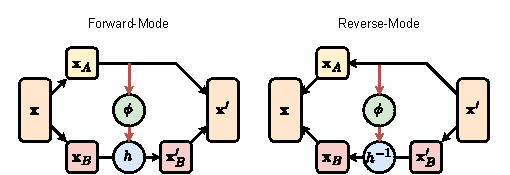
\includegraphics[width=0.8\textwidth]{Figures/generative_models/coupling.pdf}
    \caption{A diagram of a coupling flow.}
    \label{fig:coupling_flow}
\end{figure}

Note that the layer only transforms $\x_B$, leaving $\x_A$ unchanged.
Thus, multiple coupling layers are typically stacked together and interleaved with a fixed random permutation layer or a linear flow to mix the elements of $\x$.
Equivalently, one could also alternate the mask used to partition $\x$ between coupling layers.
Setting $h$ as an elementwise transformation is standard to ensure efficiency.
Early original coupling flows used an affine transformation for $h$~\cite{RealNVP}, which required many layers to fit complex data distributions.
The expressivity of the model can be significantly enhanced using more complex transformations, yet still elementwise bijections, such as rational quadratic splines~\cite{NeuralSplineFlows}.
Splines are especially useful for modelling multimodal data distributions, as single segments within the monotonic splines can become arbitrarily steep, allowing for regions of very low density.
This is demonstrated by \Cref{fig:samples}, which shows the output of a flow with four coupling layers with spline transformations.
The learned densities are shown in \Cref{fig:density}.

\begin{figure}[ht]
    \centering
    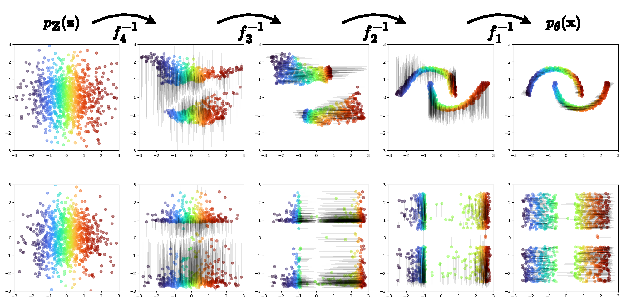
\includegraphics[width=0.95\textwidth]{Figures/generative_models/samples.pdf}
    \caption{The transformation of Gaussian samples into a double-moon distribution (top) and a four-box distribution (bottom) using a flow with 4 coupling layers. Each coupling layer can only transform one dimension of the data.}
    \label{fig:samples}
\end{figure}

\begin{figure}[ht]
    \centering
    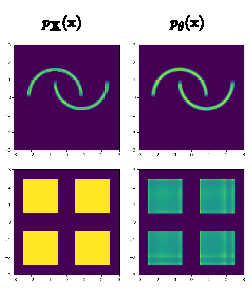
\includegraphics[width=0.4\textwidth]{Figures/generative_models/densities.pdf}
    \caption{The learned (left) and real (right)densities of the double-moon distribution (top) and the four-box distribution (bottom) using a NF.}
    \label{fig:density}
\end{figure}

\subsubsection{Autoregressive Flows}

An autoregressive model is a model decomposes the joint probability distribution into a set of conditional probabilities following a fixed order using the chain rule of probability,
\begin{equation}
    p(\x) = \prod_{i=1}^d p(x_i | x_{<i}).
\end{equation}
In a flow this can be used to define a layer that transforms the data sequentially, where the transformation of each element is conditioned on those previous.
This is called an autoregressive flow~\cite{MaskedAutoregressiveFlow}.
Like a coupling layer, there are two distinct types of transformations in an autoregressive flow, the elementwise transformation $h$ and the conditioning transformation $\phi$.
However, in this case there are $d$ different $\phi$ functions, one for each vector with $d$ elements.
The transformation for the $i$th element is given by,
\begin{equation}
    \label{eq:autoregressive_flow}
    f(\x)_i = h(x_i; \phi_i(x_{<i})).
\end{equation}
The elementwise transformation $h$ are typically the same as those used in coupling layers.
The Jacobian of this transformation is clearly triangular, thus the determinant is simply the product of the diagonal elements,
\begin{equation}
    \det D f(x) = \prod_{i=1}^d \frac{\partial h(x_i; \phi_i(x_{<i}))}{\partial x_i}.
\end{equation}
It is possible to efficiently compute the output of all $phi$ functions in parallel using a single network and a masking scheme~\cite{MADEMaskedAutoencoder}.
This means that the using the flow in forward-mode is highly efficient.
The reverse-mode however must be performed sequentially, as the transformation of each element is conditioned on the previous elements, as shown in \Cref{fig:autoregressive_flow}.
This makes autoregressive flows fast for training but slow for sampling.
Alternatively one could parametrize the layer inversely, choosing efficient sampling but slow training~\cite{ImprovingVariationalInference}.

\begin{figure}[ht]
    \centering
    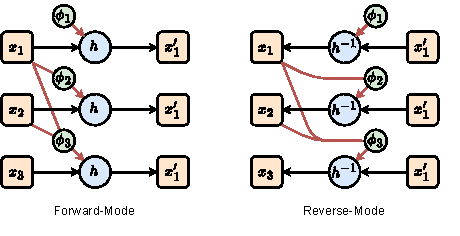
\includegraphics[width=0.8\textwidth]{Figures/generative_models/autoreg.pdf}
    \caption{A diagram of an autoregressive flow. The forward-mode transformation (left) can be computed in parallel, while the reverse-mode transformation (right) must be computed sequentially.}
    \label{fig:autoregressive_flow}
\end{figure}

\subsection{Continuous Normalizing Flows}

Whereas in a standard NF, the transformation is composed of a fixed number of sub-transformations or flow layers, a continuous normalizing flow (CNF)~\cite{NeuralODE} defines a continuous process where each infinitesimal transformation depends on the current state of the data and the time index.
This leads to an ordinary differential equation (ODE) of variable $\x_t \in \mathbb{R}^d$ indexed by $t \in [0, 1]$ defined by a smooth time-varying vector field $u(\x_t, t)$\footnote{We will use $u_t(\x_t)$ and $u(\x_t, t)$ interchangeably.},
\begin{equation}
    \label{eq:cnf}
    \diff \x_t = u_t(\x_t) \diff t.
\end{equation}
Given $\x_0 \sim p_0$, the vector field creates a pushforward $p_t = [\phi_t]_\# p_0$, where $\phi_t$ is the solution of the ODE,
\begin{equation}
    \label{eq:cnf_pushforward}
    \x_t = \phi_t(\x_0) = \x_0 + \int_0^t u_s(\x_s) \diff s.
\end{equation}
The time-dependant density $p_t(\x_t)$ must satisfy the continuity equation,
\begin{equation}
    \label{eq:cnf_continuity}
    \frac{\partial p_t}{\partial t} = -\nabla \cdot (u_t p_t).
\end{equation}
The velocity field $u_t$ is said to be the \textit{probability flow} ODE~\cite{ScoreBasedGenerativeModeling} and $p_t$ is the \textit{probability path} generated by $u_t$.
The induced log-likelihood of the pushforward is given by,
\begin{equation}
    \label{eq:cnf_loglikelihood}
    \log p_t(\x_t)
    = \log p_0(\x_0) - \int_0^t Tr\left(D u_s(\x_s)\right)\diff s
    = \log p_0(\x_0) - \int_0^t (\nabla \cdot u_s)(\x_s) \diff s,
\end{equation}
where $Tr$ is the trace operator.
This relationship was proven in \textcite{NeuralODE}.

To make this model generative, one can set the end-points of the probability path to be the data distribution $p_1 = p_\X$ at $t=1$ and the latent distribution $p_0 = p_\Z$ at $t=0$.
A neural network is then used to learn the velocity field $u_\theta(\x, t): \mathbb{R}^d \times \mathbb{R}_{+} \rightarrow \mathbb{R}^d$ allowing one to interpolate between the two via \Cref{eq:cnf_pushforward}.

Like any flow, the CNF can be trained by maximizing the log-likelihood of the data,
\begin{equation}
    \label{eq:cnf_loss}
    \mathcal{L}(\theta) = \mathbb{E}_{\x \sim \mathcal{D}}\left[\log p_0(\x) - \int_0^1 (\nabla \cdot u_\theta(\x_t, t)) \diff t\right].
\end{equation}
Once the transformation is defined, any numerical ODE solver can transform samples from the data space to the latent space and back again.
This introduces an extra level of complexity when evaluating the model.
A single trained model can have a wide range of behaviour depending on the choice of ODE solver, the number of integration steps, or the use of adaptive step sizes.
With fewer steps, truncation errors during generation can lead to a loss of sample quality, but with more steps, the computational cost of generation increases.

CNFs are highly expressive models but are slow to train.
The loss requires calculating the divergence of the vector field, which is slow to compute in many libraries\footnote{Libraries with advanced automatic differentiation, like JAX\cite{JAX}, can alleviate this issue to a degree}.
Some practical models for low dimensions utilise the Hutchinson trace estimator~\cite{FFJORD},  approximating the trace of the Jacobian with a single Monte Carlo sample.
Even with these optimizations, a single training iteration still requires a full numerical integration of the ODE and subsequent backpropagation through each step, making CNFs impractical for high-dimensional data.


\section{Diffusion Models}

Over the past four years, diffusion models have emerged as the standard for generating high-dimensional data.
Their impact on the landscape of PGMs has been profound.
They have elevated the field from method papers on two-dimensional toy datasets to commercially viable high-resolution text-to-image models which are now flooding the internet.
This significant advancement is primarily due to the exceptionally straightforward training of diffusion models, especially compared to CNFs and GANs.
Their training process is largely stable, with fixed supervised targets.
Furthermore, diffusion models allow for seamless incorporation of contextual generation, enabling fine control over the generated samples.
Finally, the quality of the samples drawn from a diffusion model outperforms all other PGMs.

Diffusion models emerged in 2015~\cite{DeepUnsupervisedLearning}, where the authors were inspired by non-equilibrium statistical physics.
There are three main components to this type of model.
The first is a forward-process that iteratively and systematically destroys structured data by adding noise.
Typically, this is non-learnable and simple to compute.
By the end of the process, any structure is destroyed, and the sample is indistinguishable from pure noise.
A model is trained to learn the reverse-process, which restores the data structure in a similarly iterative scheme.
Generation involves taking a sample of pure noise, typically $\normal$,  and repeatedly applying the reverse-process to modify it into a sample that matches the data distribution.
This defines the final component, the \textit{sampling procedure}, a single trained model can be sampled in many ways, which present trade-offs between speed and quality.
Between 2015 and 2019, the method was largely overlooked, then
In 2020, it was revisited, improved, and applied successfully to images in the form of the Diffusion Probabilistic Models (DDPM)~\cite{DDPM}.
The true research frenzy began in 2021 when diffusion models officially dethroned GANs as the state-of-the-art for conditional image generation~\cite{DiffusionBeatsGANS}.

Many competing, overlapping, and sometimes equivalent frameworks are used to define diffusion models.
They are described through the lens of Markov chains trained via variational inference~\cite{DDPM, DDIM}, score-based models with Langevin Dynamics~\cite{ScoreBasedGenerativeModeling, ElucidatingDesignSpace}, and flow matching with CNFs~\cite{BuildingNormalizingFlows, FlowMatchingGenerative, FlowStraightFast}.
These models share similar training objectives but differ in the mathematical derivations.
Many attempts have been made to unify these models under a framework~\cite{CM2, ElucidatingDesignSpace, UnderstandingDiffusionModels, StochasticInterpolants, FlowStraightFast}.
Since no single framework has emerged as the standard, we will not attempt to unify them here.
However, this chapter uses the term ``diffusion model'' as an umbrella term to describe all of these models, and we chose to focus on two frameworks that are used directly in the projects of this thesis, namely score-based models~\cite{ScoreBasedGenerativeModeling} and flow matching models~\cite{BuildingNormalizingFlows, FlowMatchingGenerative, FlowStraightFast}.

\subsection{Score-Based Generative Models}
\label{sec:score_based}

Score-based generative modelling~\cite{ScoreMatching, ScoreBasedGenerativeModeling} is a framework that envelops many diffusion models such as DDPM~\cite{DDPM}.
The forward-process involves progressively applying Gaussian perturbations to a data sample in the continuous such that it can be modelled as an SDE,
\begin{equation}
    \label{eq:sde}
    \diff \x_t = \underbrace{f(\x_t, t)}_{\mathclap{\text{drift}}} \diff t + \underbrace{g(t)}_{\mathclap{\text{diffusion}}} \diff \w_t,
\end{equation}
where $\w_t$ is the standard Wiener process (Brownian motion) and $f: \mathbb{R}^d \times \mathbb{R}_{+} \rightarrow \mathbb{R}^d$, $g: \mathbb{R}_{+} \rightarrow \mathbb{R}$ are the drift and diffusion functions respectively, and $t \in [0, T]$ is the time index.
At $t=0$, the sample is uncorrupted\footnote{Note that the time index in diffusion models is typically inverted compared to CNFs}.
Note that if $|g(t)| > 0$ the data signal is progressively corrupted.

While the forward-process is non-learnable, it is not quick to solve without numerical integration.
However, if the drift function is affine with respect to $\x_t$, the transition kernel becomes Gaussian,
\begin{equation}
    \label{eq:gaussian_kernel}
    f(\x_t, t) = f(t)\x_t \quad \Rightarrow \quad p_{0t}(\x_t|\x_0) = \mathcal{N}(\x_t; s(t)\x_0, \sigma(t)^2 \mathbb{I}),
\end{equation}
where $s(t)$ and $\sigma(t)$ are time-dependent scaling factors, referred to as the \textit{signal rate} and \textit{noise rate} respectively, and can be derived for specific forms of $f(t)$ and $g(t)$~\cite{sarkka2019applied}.
Alternatively one can select specific forms for the scaling factors and derive the drift and diffusion functions~\cite{ElucidatingDesignSpace}.
Either way, this choice uniquely defines the \textit{diffusion schedule} for the process, and for generative models one typically constructs it such that,
\begin{equation}
    \label{eq:diffusion_schedule}
    \lim_{t \rightarrow 0} s(t) = 1, \quad \lim_{t \rightarrow 0} \sigma(t) = 0, \quad \lim_{t \rightarrow T} \frac{s(t)}{\sigma(t)} = 0,
\end{equation}
as this ensures that time-dependant marginal of the distribution follows $p_0 = p_\X$ and that $p_\Z \approx p_T = \mathcal{N}(0, \sigma(T) \mathbb{I})$.
Using the transition kernel defined in \Cref{eq:gaussian_kernel}, one is able to sample from the forward-process at any arbitrary time $t$ using the reparametrization trick,
\begin{equation}
    \label{eq:reparametrization}
    \x_t = s(t)\x_0 + \sigma(t) \z \quad \text{where} \quad \z \sim \normal \quad \text{and} \quad \x_0 \sim p_0(\x).
\end{equation}

Remarkably, the SDE in \Cref{eq:sde} has an exact inverse~\cite{ReversetimeDiffusionEquation} which can be used to define the reverse-process,
\begin{equation}
    \label{eq:reverse_sde}
    \diff \x_t = \left[ f(\x_t, t) - g(t)^2 \score \right] \diff t + g(t) \diff \bar\w_t,
\end{equation}
where $\bar\w_t$ is a Wiener process with opposing sign and time flows from $T \rightarrow 0$.
The only unknown term in \Cref{eq:reverse_sde}, $\score$, is referred to as the score function and thus approximating it, called score matching (SM), is the main objective of a score-based generative model.

One naive approach to perform SM is to use direct regression via mean-squared-error which results in the loss function,
\begin{equation}
    \label{eq:naive_loss}
    \mathcal{L}_{SM}(\theta) =
    \mathbb{E}_{t \sim \unitime}
    \mathbb{E}_{\x_t \sim p_t(\x_t)}
    \left|\left|S_\theta(\x_t, t) - \score\right|\right|^2,
\end{equation}
where $S_\theta$ is a neural network with trainable parameters $\theta$.
However, this loss is not practical as it requires the calculation of the very term we are trying to approximate.
One can instead use the denoising score matching (DSM) objective~\cite{ScoreMatching, SlicedScoreMatching} where the conditional score function $\cscore$ is approximated,
\begin{equation}
    \label{eq:denoising_loss}
    \mathcal{L}_{DSM}(\theta) =
    \mathbb{E}_{t \sim \unitime}
    \mathbb{E}_{\x_0 \sim \mathcal{D}}
    \mathbb{E}_{\x_t \sim p_{0t}(\x_t|\x_0)}
    \left|\left|S_\theta(\x_t, t) - \cscore\right|\right|^2.
\end{equation}
This replacement is valid because after taking all expectations, the gradients of the two loss functions are equivalent with respect to the model parameters~\cite{ScoreBasedGenerativeModeling},
\begin{equation}
    \nabla_{\theta} \mathcal{L}_{SM}(\theta) = \nabla_{\theta} \mathcal{L}_{DSM}(\theta).
\end{equation}
This replacement is useful because the conditional score function does have a tractable form due to the transition kernel in \Cref{eq:gaussian_kernel},
\begin{equation}
    \begin{aligned}
        \label{eq:conditional_score}
        \cscore
         & = -\nabla_{\x_t} \log \left( \mathcal{N}(\x_t; s(t)\x_0, \sigma(t)^2 \mathbb{I}) \right) \\
         & = -\nabla_{\x_t} \frac{\left(\x_t - s(t)\x_0\right)^2}{2\sigma(t)^2}                     \\
         & = \frac{s(t)\x_0 - \x_t}{\sigma(t)^2}                                                    \\
         & = \frac{s(t)\x_0 - s(t)\x_0 - \sigma(t)\z}{\sigma(t)^2}                                  \\
         & = - \frac{\z}{\sigma(t)},
    \end{aligned}
\end{equation}
where we have also applied the reparametrization trick from \Cref{eq:reparametrization}.
It is convenient to precondition the network output as,
\begin{equation}
    \label{eq:precondition}
    S_\theta(\x_t, t) = - \frac{z_\theta(\x_t, t)}{\sigma(t)},
\end{equation}
yielding the final loss function,
\begin{equation}
    \label{eq:noise_loss}
    \mathcal{L}_{DSM}(\theta) =
    \mathbb{E}_{t \sim \unitime}
    \mathbb{E}_{\x_0 \sim \mathcal{D}}
    \mathbb{E}_{\z \sim \normal}
    \frac{\gamma(t)}{\sigma(t)^2}
    \left|\left|z_\theta(\x_t, t) - \z\right|\right|^2.
\end{equation}
Here, $\gamma(t) > 0$ is introduced as a reweighting factor to balance the loss across the time domain.
Note that by setting $\gamma(t) = \sigma(t)^2$ the loss is uniformly weighted and this often corresponds to good perceptual quality of the generated samples~\cite{VariationalPerspectiveDiffusionBased, VariationalDiffusionModels, ImprovedDenoisingDiffusion}.
Alternatively, one can use specific weighting schemes to allow training on the maximum likelihood objective~\cite{UnderstandingDiffusionModels}.

Once the model is trained, one can define the sampling procedure, which starts from samples drawn from $p_Z=\mathcal{N}(0, \sigma(T) \mathbb{I})$ and numerically integrates the reverse SDE in \Cref{eq:reverse_sde} from $t: T \rightarrow 0$ to obtain samples matching $p_0$.
The integration can be done using the Euler-Maruyama method or stochastic Runge-Kutta methods~\cite{NumericalSolutionStochastic}.
Like CNFs, the generation quality is highly sensitive to the number of integration steps as each step requires another forward pass through the neural network.
The high computational cost of generating a sample with a diffusion model is the main drawback of this approach compared to single-pass methods like NFs and GANs.

As a method to speed up generation, \textcite{ScoreBasedGenerativeModeling} proved the existence of the probability flow ODE whose solutions share the same marginal densities $p_t(\x_t)$ as the SDE.
For the SDE defined in \Cref{eq:sde} it is given by,
\begin{equation}
    \label{eq:probability_flow}
    \diff \x_t = \left[f(\x_t, t) - \frac{1}{2} g(t)^2 \score\right] \diff t.
\end{equation}
Empirically, the probability flow ODE provides a larger tolerance to truncation errors, allowing for fewer integration steps and, thus, faster generation.
In addition, it enables the use of more advanced ODE solvers, provides deterministic encoding, and allows for log-likelihood computation via~\Cref{eq:cnf_loglikelihood}, indicating the strong connection between score-based models and CNFs.
Furthermore, while the probability flow ODE was initially introduced as an alternative method for generation, \textcite{ElucidatingDesignSpace} showed that the entire training objective of a score-based model can be derived purely from an ODE perspective.

\subsection{Conditional Flow Matching}
\label{sec:cfm}

Conditional Flow Matching (CFM)~\cite{BuildingNormalizingFlows, FlowMatchingGenerative, FlowStraightFast} is an alternative framework which arrives at an equivalent training objective to score-based models and can be seen as a method to construct CNFs without the need for numerical integration during training.
The derivation shares many parallels with score-based models, and abundant literature argues their equivalence~\cite{CM2, StochasticInterpolants}.
However, they approach the problem without using SDEs, and like \textcite{ElucidatingDesignSpace}, directly target the probability flow ODE, arguably yielding a more straightforward derivation.

Like CNFs, the goal of CFM is to learn the velocity field $u_t(\x_t)$ that induces the time-dependent density $p_t(\x_t)$ adhering to the boundary conditions $p_1 = p_\X$ and $p_0 = p_\Z$\footnote{Note again that the time index is inverted compared to score-based models.}.
One can express this density as a marginal over a conditional probability path which propagates from a single data sample,
\begin{equation}
    \label{eq:conditional_path}
    p_t(\x_t) = \int p_1(\x_1) p_{t1}(\x_t|\x_1) \diff \x_1.
\end{equation}
The conditional probability path has the endpoints,
\begin{equation}
    \label{eq:conditional_path_endpoints}
    p_{01}(\x_t|\x_1) = p_0(\x_t) \quad \text{and} \quad p_{11}(\x_t|\x_1) = \delta(\x_t - \x_1),
\end{equation}
and is generated by its own conditional vector field $u_t(\x_t | \x_1)$ with the consistency condition,
\begin{equation}
    \label{eq:conditional_consistency}
    \frac{\partial p_{t1}(\x_t | \x_1)}{\partial t} = -\nabla \cdot (u_t(\x_t | \x_1) p_{t1}(\x_t | \x_1)).
\end{equation}

The conditional vector field $u_t(\x_t | \x_1)$ can be used to express the marginal vector field $u_t(\x_t)$ as,
\begin{equation}
    \label{eq:conditional_to_marginal}
    u_t(\x_t) = \int u_t(\x_t | \x_1) \frac{p_{t1}(\x_t | \x_1) p_1(\x_1)}{p_t(\x_t)} \diff \x_1.
\end{equation}
This is proven by,
\begin{equation}
    \begin{aligned}
        \frac{\partial p_t(\x_t)}{\partial t}
         & = \frac{\partial}{\partial t} \int p_{t1}(\x_t | \x_1) p_1(\x_1) \diff \x_1                                                            \\
         & = \int \frac{\partial}{\partial t} p_{t1}(\x_t | \x_1) p_1(\x_1) \diff \x_1                                                            \\
         & = - \int \left(\nabla \cdot (u_t(\x_t | \x_1) p_{t1}(\x_t | \x_1))\right) p_1(\x_1) \diff \x_1                                         \\
         & = - \nabla \cdot \left(\int u_t(\x_t | \x_1) p_{t1}(\x_t | \x_1) p_1(\x_1) \diff \x_1\right)                                           \\
         & = - \nabla \cdot \left(\int u_t(\x_t | \x_1) \frac{p_{t1}(\x_t | \x_1) p_1(\x_1)}{p_t(\x_t)} p_t(\x_t) \diff \x_1\right)               \\
         & = - \nabla \cdot \left(\left(\int u_t(\x_t | \x_1) \frac{p_{t1}(\x_t | \x_1) p_1(\x_1)}{p_t(\x_t)} \diff \x_1\right) p_t(\x_t) \right) \\
         & = - \nabla \cdot \left(u_t(\x_t) p_t(\x_t)\right),
    \end{aligned}
\end{equation}
which is the continuity equation for the marginal density $p_t(\x_t)$.
With these relations we can apply the same trick we did for score-matching, in that the flow matching (FM) loss,
\begin{equation}
    \label{eq:fm_loss}
    \mathcal{L}_{FM}(\theta) =
    \mathbb{E}_{t \sim \timeone}
    \mathbb{E}_{\x_t \sim p_t(\x_t)}
    \left|\left|u_\theta(\x_t) - u_t(\x_t)\right|\right|^2,
\end{equation}
and the CFM loss,
\begin{equation}
    \label{eq:cfm_loss}
    \mathcal{L}_{CFM}(\theta) =
    \mathbb{E}_{t \sim \timeone}
    \mathbb{E}_{\x_1 \sim \mathcal{D}}
    \mathbb{E}_{\x_0 \sim p_0}
    \left|\left|u_\theta(\x_t, t) - u_t(\x_t | \x_1)\right|\right|^2,
\end{equation}
are equivalent with respect to the model parameters $\nabla_{\theta} \mathcal{L}_{FM}(\theta) = \nabla_{\theta} \mathcal{L}_{CFM}(\theta)$~\cite{FlowMatchingGenerative}.

The only remaining feature is to describe the conditional probability path $p_{t1}(\x_t | \x_1)$.
The authors of~\cite{FlowStraightFast} propose a basic Gaussian probability path,
\begin{equation}
    \label{eq:conditional_gaussian}
    p_{t1}(\x_t | \x_1) = \mathcal{N}(\x_t; (1 - t)\x_1, t^2\mathbb{I}),
\end{equation}
which matches the relation in \Cref{eq:gaussian_kernel} by setting $s(t) = 1 - t$ and $\sigma(t) = t$ and allows for the same reparametrization trick for sampling.
This choice is often referred to as the linear interpolation scheme and corresponds to the conditional vector field,
\begin{equation}
    \label{eq:conditional_gaussian_field}
    u_t(\x_t | \x_1) = \frac{\x_t-\x_1}{t}.
\end{equation}
Under the linear interpolation scheme \Cref{eq:cfm_loss} simplifies even further to,
\begin{equation}
    \label{eq:linear_cfm_loss}
    \mathcal{L}_{CFM}(\theta) =
    \mathbb{E}_{t \sim \timeone}
    \mathbb{E}_{\x_1 \sim \mathcal{D}}
    \mathbb{E}_{\x_0 \sim p_0}
    \left|\left|u_\theta(\x_t, t) - (\x_1 - \x_0)\right|\right|^2,
\end{equation}
which is the most common form of the loss used in practice.

Once the network is trained, one can sample from the model by integrating the conditional vector field from noise sample to the data sample as with any CNF.

\subsection{Diffusion Models in Practice}

The training step for most diffusion models is essentially the same.
One samples a time index $t$, a data point $\x \sim p_\X$, and a latent variable $\z \sim p_\Z$.
They are then mixed to get the partially noised sample $\x_t = s(t)\x + \sigma(t)\z$ using predefined scaling factors and passed along with the time index to a neural network.
The network is trained to predict the noise, data point, or velocity field directly.
A trained network defines the ODE or SDE, which can be used to generate samples via numerical integration.
Specifics in this process depend on the choice of framework, the network architecture, and the hyperparameters used.

Over the past four years, some best practices have emerged for training and sampling from diffusion models, such as using slow moving offline networks, targeted time sampling, time encoding, and more advanced ODE solvers.

\subsubsection{Diffusion Frameworks}
\label{sec:diffusion_frameworks}

Three diffusion frameworks are used in the various projects within this thesis.
The first uses the SM objective by~\textcite{GenerativeModelingEstimating} with trigonometric interpolations~\cite{StochasticInterpolants, ImprovedDenoisingDiffusion}, which we refer to as SM-TI, the second follows the work by~\textcite{ElucidatingDesignSpace} often referred to as EDM diffusion, and the third is the CFM framework by~\textcite{FlowMatchingGenerative, FlowStraightFast, BuildingNormalizingFlows}.
We briefly summarize the main differences in the hyperparameters used in each framework in \Cref{tab:diffusion_frameworks}.

In SM-TI, the diffusion schedule is chosen to be a cosine and sine function such that the total power of $\x_t$, assuming that the training set was standardized, is constant across the schedule.
The network predicts the noise added to the data with the training objective
$\mathbb{E}_{\x, \z, t} \lambda(t) \left|\left| z_\theta(\x_t, t) - \z\right|\right|^2$.
This is then used to approximate the score function, which is used in either the reverse SDE or the probability flow ODE to generate samples.

In EDM, the diffusion schedule is constructed to simplify the form of the probability flow ODE as much as possible.
Noise is added at a linearly increasing rate to a signal that is kept constant, $\x_t = \x_0 + t\z$.
This results in an ODE with straighter trajectories, which is beneficial for the numerical integration during sampling as it reduces the truncation errors.
The time domain extends to $t_\text{max}$, which also determines the latent distribution's variance and is typically set to be $t_\text{max} = 80$.
The objective is to predict the data itself, with the loss $\mathbb{E}_{\x, \z, t} \lambda(t) \left|\left| x_\theta(\x_t, t) - \x\right|\right|^2$.
The actual network is preconditioned such that
\begin{equation}
    x_\theta = c_\text{skip}(t) \x_t + c_\text{out}(t)f_\theta(c_\text{in}(t)\x_t, c_\text{noise}(t)),
\end{equation}
where $f_\theta$ is the neural network and $(c_\text{skip}, c_\text{in}, c_\text{out}, c_\text{noise})$ are scaling factors.
These factors are manually selected such that the training objective and the network's inputs have unit variance across all values of $t \in [0, t_\text{max}]$.
One can take steps towards the estimated data sample during integration with any ODE.
While this loss was derived without the need for an SDE, the authors of EDM also showed that using a stochastic sampler can improve the quality of the generated samples if enough integration steps are taken.

The CFM framework follows the derivation in \Cref{sec:cfm}, where the diffusion schedule is a basic linear interpolation between the noise and the data and the network target is simply the difference between the two.
CFM has arguably the simplest to implement training loop, which is shown in \Cref{code:cfm}.
This model generated the samples in \Cref{fig:cm_samples}, which includes double-moon and four-box datasets.
One of the main benefits of the CNF framework is that the latent distribution does not have to be Gaussian, and the theory holds for any arbitrary distributions.
The bottom row of \Cref{fig:cm_samples} has the model interpolating from the double-moon distribution to the four-box distribution.

\begin{figure}
    \centering
    \scriptsize
    \begin{minted}{python}
    class CFM(nn.Module):
        def __init__(self, dim, time_dim):
            super().__init__()
            self.mlp = MLP(input_dim=dim, output_dim=dim, context_dim=time_dim)
            self.cos_enc = CosEnc(dim, time_dim)

        def get_loss(self, x0):
            t = T.rand((x0.size(0), 1))                # Sample time
            x1 = T.randn_like(x0)                      # Sample noise
            xt = (1 - t) * x0 + t * x1                 # Linear interpolation
            ut = self.mlp(xt, self.cos_enc(t))         # Predict velocity
            return (ut - (x0 - x1)).square().mean()    # MSE loss
    \end{minted}
    \caption{A simple implementation of the CFM framework in PyTorch. The model is trained to predict the velocity field $u_t(\x_t)$ that interpolates between noise $\x_1$ and data $\x_0$ at time $t$.}
    \label{code:cfm}
\end{figure}

A natural question arises regarding which of these models performs better.
Research on this topic is ongoing, and the community has yet to reach a consensus.
However, the CFM framework with the linear interpolation diffusion schedule is now used by the majority of commercial diffusion models for text-to-image synthesis.
This includes models such as Stable Diffusion 3~\cite{SD3} and Flux~\cite{flux2024github}, indicating a practical preference for this framework.

    {
        \renewcommand{\arraystretch}{1.5}
        \begin{table}[h!]
            \centering
            \caption{Hyperparameters used in the different diffusion frameworks.}
            \label{tab:diffusion_frameworks}
            \resizebox{\textwidth}{!}{
                \begin{tabular}{cccc}
                    \toprule
                                                 & \textbf{SM-TI}                                        & \textbf{EDM}                               & \textbf{CFM}           \\
                    \midrule
                    time index $t$               & $t \in [0, 1]$                                        & $t \in [0, t_{max}]$                       & $t \in [0, 1]$         \\
                    signal rate $s(t)$           & $\cos(\frac{t\pi}{2})$                                & $1$                                        & $1 - t$                \\
                    noise rate $\sigma(t)$       & $\sin(\frac{t\pi}{2})$                                & $t$                                        & $t$                    \\
                    latent distribution          & $\normal$                                             & $\mathcal{N}(0, t_\text{max}^2\mathbb{I})$ & $\normal$              \\
                    training target              & noise - $\z$                                          & data - $\x$                                & velocity - $(\x - \z)$ \\
                    $\frac{\diff \x_t}{\diff t}$ & $- \frac{\pi}{2}\tan(\frac{\pi t}{2})(\x_t - \score)$ & $- t \score$                               & $u_t(\x_t)$            \\
                    sampling                     & SDE or ODE                                            & SDE or ODE                                 & ODE                    \\
                    \bottomrule
                \end{tabular}
            }
        \end{table}
    }

\begin{figure}[ht]
    \centering
    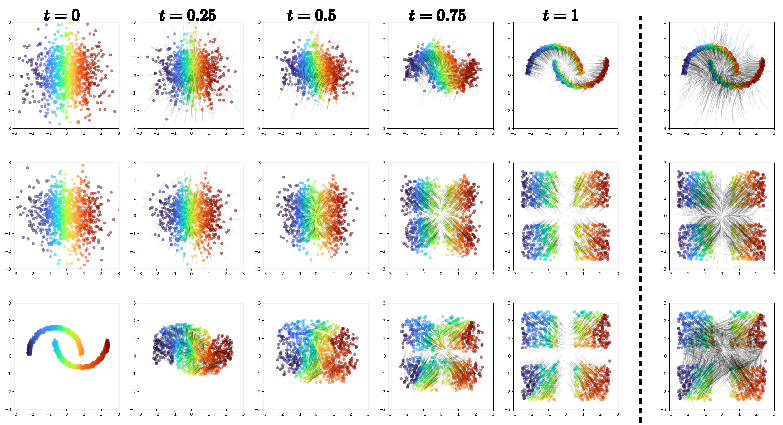
\includegraphics[width=0.99\textwidth]{Figures/generative_models/cm_samples.pdf}
    \caption{The transformation of Gaussian samples into a double-moon distribution (top) and a four-box distribution (middle), and the interpolation between the two (bottom). The model was trained using the CNF framework generated with Heun's method~\cite{heun} for 64 steps. Each column shows the samples at a different time index $t$, the black lines trace back to the samples in the previous column. The rightmost column shows the full paths traced by each sample from the base distribution.}
    \label{fig:cm_samples}
\end{figure}


\subsubsection{Conditional Verses Unconditional Paths}

One of the claims of both EDM and CFM is that they lead to straighter trajectories than SM-TI, allowing for faster sampling as fewer steps are needed in the numerical integration.
This is indeed the case, as shown by \Cref{fig:vp_vs_cfm}, where the SM-TI model results in paths with very high curvature, especially at the end of the schedule.
Note that none of the paths are completely straight.
This is because all frameworks were derived using a similar technique to overcome the intractable marginal density (velocity) by using the conditional density (conditional velocity) as a proxy.
This means tension exists between the actual training target and what the model approximates, and this discrepancy is highlighted in \Cref{fig:oned_oned}.
In the latter case, the model was trained to interpolate between samples drawn from the same distribution, meaning that an optimal model would be $u_t(\x_t) = 0$
So, even if the conditional paths are straight, as with EDM and CFM, the marginal paths are not.
This discrepancy results in a few considerations for training.

\begin{figure}[ht]
    \centering
    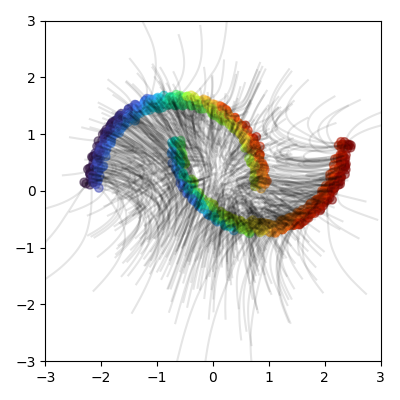
\includegraphics[width=0.45\textwidth]{Figures/generative_models/fm.png}
    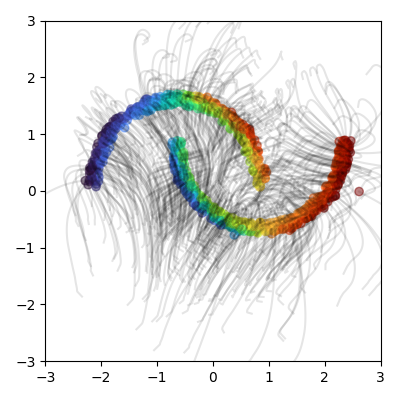
\includegraphics[width=0.45\textwidth]{Figures/generative_models/vp.png}
    \caption{The marginal paths generated interpolating between a Gaussian and a double-moon distribution learned by using the CFM schedule (left) and the SM-TI schedule (right).}
    \label{fig:vp_vs_cfm}
\end{figure}

Using conditional paths as a proxy training target results in unbiased updates with high variance.
While diffusion models are not at risk of collapsing like GANs, gradient updates are highly stochastic, and convergence is slow.
Almost all diffusion models are trained with two copies of the network: an online-network and an offline-network.
The online-network is updated using standard gradient descent, while the offline network is updated using the exponential moving average (EMA) of the online network.
The offline-network is always used for sampling.
This common trick could be applied to any deep learning task~\cite{Adam}, but it is ubiquitous in diffusion models.

Note that predicting the marginal velocity for CFM is significantly harder in the middle of the schedule than at the endpoints.
This is because the optimal prediction for the marginal velocity at $t=0$ is a vector pointing towards the mean of $p_1$, and the optimal prediction at $t=1$ points towards the mean of $p_0$.
Similarly, at $t=t_0$ in EDM, $f_\theta$ should be the identity function, and at $t=t_\text{max}$, the ideal denoiser returns the mean of the training set.
Therefore, it is common to use non-uniform sampling for the time index during training to target the time steps where the most information can be gained.
These are typically based on empirical results and are not derived from the theory.
For EDM, $\log(t) \sim \mathcal{N}(-1.2, 1.2)$ was chosen after a hyperparameter search and for CFM it was found that logit-normal sampling,
\begin{equation}
    t \sim \frac{1}{\sqrt{2\pi}}\frac{1}{t(1-t)}\exp\left(-\frac{(\text{logit}(t))^2}{2}\right),
\end{equation}
where $\text{logit}(t) = \log\left(\frac{t}{1-t}\right)$, was the most effective~\cite{SD3}.

\begin{figure}[ht]
    \centering
    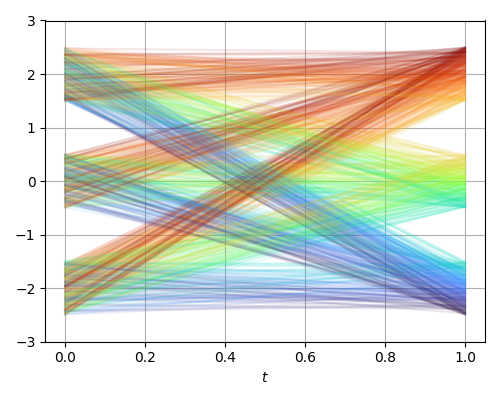
\includegraphics[width=0.49\textwidth]{Figures/generative_models/oned2.png}
    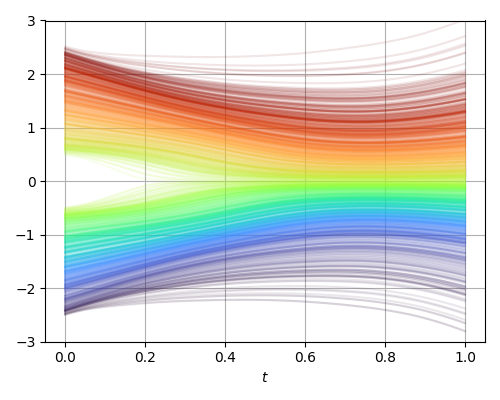
\includegraphics[width=0.49\textwidth]{Figures/generative_models/oned.png}
    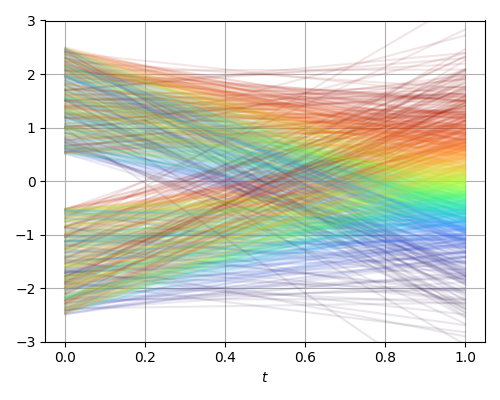
\includegraphics[width=0.49\textwidth]{Figures/generative_models/oned_target.png}
    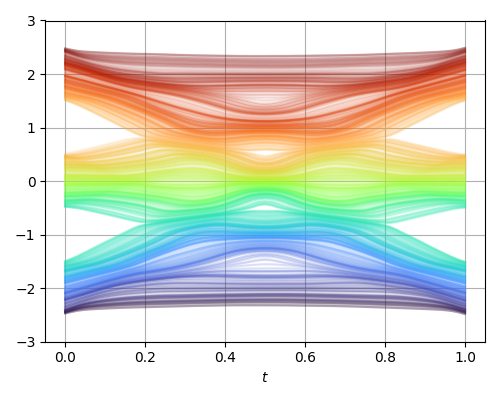
\includegraphics[width=0.49\textwidth]{Figures/generative_models/oned2_marginal.png}
    \caption{(left) The conditional paths used to train a CFM, and (right) the marginal paths generated by the model. The top row shows a model interpolating between a two-box distribution and a Gaussian distribution, and the bottom row shows a model interpolating between samples drawn from the same three-box distribution.}
    \label{fig:oned_oned}
\end{figure}

\subsubsection{Straighter Paths and Distillation}

Even with the aforementioned training tricks, the highly variant outputs are still a problem, and much work has been dedicated to learning straighter paths.
Straight paths would be optimal, as they could be solved using a single Euler step.
One approach is to use mini-batch optimal transport couplings between the data and the latent samples before mixing~\cite{ImprovingGeneralizingFlowbased}.
However, this method does not scale well to high-dimensional data, even for mini-batches.
Another approach is to take a trained model and \textit{distil} it by training a second model to learn the same endpoints as the first model but with straighter trajectories.
There are various methods for distillation, such as rectification~\cite{FlowStraightFast}, progressive distillation~\cite{ProgressiveDistillationFast}, and consistency distillation~\cite{ConsistencyModels}.
Each method attempts to reduce the number of inference steps required to generate high-quality samples.

However, there is an argument to be made that the multiple steps make diffusion models so powerful.
Since the process requires removing noise from the data, any additional error terms induced by truncation errors are also removed.
Diffusion models have been described as applying iterative refinements~\cite{ImageSuperResolutionIterative} to the data, and the multiple steps might allow the model to self-correct.

\subsubsection{Time Encoding}
\label{sec:time_encoding}

In all models, the network needs to take in time information.
One can do this by simply concatenating the time index to the input, but it is more beneficial to perform positional encoding beforehand.
This is most commonly done using trigonometric functions, such as the positional encoding used in transformers~\cite{Attention}, or random Fourier features~\cite{FourierFeaturesLet}.
However, we have found the most success with a basic cosine-encoding (CosEnc)~\cite{ImplicitQuantileNetworks}.
This layer takes a scalar $t$ and returns an output tensor of length $d$, where each element is the output of a cosine function with exponentially increasing frequency.
The lowest frequency is set such that the layer will not have duplicate outputs.
For parameters $t_\text{min}$, $t_\text{max}$, and $d$ the CosEnc layer is given by,
\begin{equation}
    \label{eq:cosine_encoding}
    \text{CosEnc}(t) =
    \begin{bmatrix}
        \cos\left(e^0 t'\right) \\
        \cos\left(e^1 t'\right) \\
        \vdots                  \\
        \cos\left(e^{d-1} t'\right)
    \end{bmatrix}, \quad \text{where} \quad t' = \pi \frac{t - t_\text{min}}{t_\text{max} - t_\text{min}}. \\
\end{equation}
This can be seen as a form of continuous binary encoding and can be used in the network layers via adaptive normalization and gating described in~\Cref{sec:global_attributes}.

\subsubsection{Conditional Generation}

Other conditioning information $\con$ can easily be added to the network, such as class labels or other auxiliary information.
This works for all frameworks and requires including the context information with the network inputs, the exact form depending on the model's architecture.
Interestingly enough, one does not even have to train a conditional model to perform conditional generation due to the relation,
\begin{equation}
    \label{eq:conditional_generation}
    \nabla_{\x_t} \cdot \log p(\x_t | \con) = \nabla_{\x_t} \cdot \log p(\x_t) + \nabla_{\x_t} \cdot \log p(\con | \x_t).
\end{equation}
Thus, one only needs a second time-dependent classifier for the conditioning information.
Gradients with respect to this model can be used to modify the update rule for the ODE or the velocity field to perform conditional generation.
This is often referred to as \textit{guidance} in the diffusion literature~\cite{DiffusionBeatsGANS}.

\subsubsection{Sampling}

As previously discussed, various numerical integration techniques can be employed with either the reverse SDE or the probability flow ODE to sample from a diffusion model.
Beyond the conventional numerical integration methods, such as Euler, Heun, and Linear Multi-Step methods~\cite{heun}, a novel domain has emerged, focusing on developing efficient integration methods tailored to specific diffusion schedules.
Notable examples include DDIM~\cite{DDIM}, DPM-Solver~\cite{DPMSolverFastODE}, DPM-Solver++~\cite{DPMSolverFastSolver}, UniPC~\cite{UniPC}, and DPM-Solver-2M~\cite{DPMSolverFastSolver}.
These samplers are adaptable to both stochastic and ordinary differential equations.

Furthermore, the number of integration steps and the step size vary across different methods. In~\cite{ElucidatingDesignSpace}, the integration steps were designed to take larger steps at the beginning of the schedule and smaller steps towards the end, facilitating refinement. This variability complicates the comparison of models, as the same model may yield different results depending on the integration method employed, presenting a significant challenge for benchmarking.

